% !TEX root = ../main.tex

\chapter{Experiments}
\label{ch:experiments}
This chapter aims to answer the research questions formulated in Section~\ref{sec:research_questions}. First, I describe which experiments I conducted. Next, I show the results of these experiments. Finally, I discuss my findings further in the last section.

\section{Experiments}
This section describes the experiments I used in order to investigate and answer the formulated research questions. We can break down the experiments into three categories: reproduction of the results of the paper \emph{Analyzing Reinforcement Learning Benchmarks with Random Weight Guessing}, comparison of the alternative models described in Section~\ref{sec:models} to neural networks, and an analysis of the impact of bias in these settings.

\subsection{Reproduction of RWG-Paper}
For a starting point, I reproduced the results of the paper \emph{Analyzing Reinforcement Learning Benchmarks with Random Weight Guessing} discussed in Section~\ref{sec:benchmarks}. I used the same methodology as the authors of the paper did. In specific, I used three network architectures: a network without any hidden layers (0 HL, 0 HU), a network with a single hidden layer of 4 units (1 HL, 4 HU), and a network with two hidden layers of 4 units each (2 HL, 4 HU). I used the same procedure as explained in pseudocode in Algorithm~\ref{alg:environment-evaluation} using RWG. I tested the three neural networks for all five classic control environments provided by the OpenAI Gym interface: \verb|CartPole|, \verb|Acrobot|, \verb|Pendulum|, \verb|MountainCar|, and \verb|MountainCarContinuous|. For the next experiments, the reproduced results serve as a guideline to judge the effectiveness of the alternative models in comparison with neural networks.
\todo[inline]{Section title good?}

\subsection{Comparison of Alternative Models to Neural Networks}
This experiment aims to provide a comparison of alternative models to the commonly used neural network model. I selected a few promising models and analyzed them with the help of the classic control environments. Analogous to the neural networks, I used three architectures for each model with increasing complexity. I conducted the following experiments:
\begin{enumerate}[label=(\alph*)]
  \item In the first experiment, I took the polynomial model $P_1$ and $P_2$ and tested them on the discrete classic control environments. I used polynomials of degrees 1, 2, and 3.
  \item In the second experiment, I tested the binary tree model on all five classic control environments. I used binary trees with 1, 4, and 8 nodes.
\end{enumerate}
I described the models in more detail in Section~\ref{sec:environments}. For the experiments, I used the same procedure as in \emph{Analyzing Reinforcement Learning Benchmarks with Random Weight Guessing} with only slight adaption. Thus, we can directly compare the results of the alternative models to those of neural networks. Another important aspect of this procedure is that there is no learning involved. For their paper, the authors were interested in the complexity of the environment, whereas I aim to find out more about the nature of the models. The classic control environments are relatively easy to solve, as explained in Section~\ref{sec:benchmarks}. Therefore, we expect some controllers to solve the task even without any learning involved.

For the experiments, first, I initialized the environment. Second, I initialized the respective model. Then, I drew the weights of the model from the standard normal distribution $\mathcal{N}(0,1)$ or the uniform distribution $U(a,b)$ depending on the model and environment used. Each of these instances of the model represents a sample. In total, I used $10'000$ samples ($N_{samples}$). Finally, I ran 20 episodes ($N_{episodes}$) with each sample for an environment and stored the respective score as an entry of the score tensor $S$. Algorithm~\ref{alg:model-evaluation} shows an overview of the described procedure. As we can see, the procedure is very similar to the one shown in Algorithm~\ref{alg:environment-evaluation}.
\begin{algorithm}
\caption{Procedure for alternative models using RWG}
\begin{algorithmic}[1]
\State Initialize environment
\State Initialize model
\State Create array $S$ of size $N_{samples} \times N_{episodes}$
\For{$n = 1,2,...,N_{samples}$}
    \State Sample model weights randomly from $\mathcal{N}(0,1)$ or $U(a, b)$
    \For{$e=1,2,...,N_{episodes}$}
      \State Reset the environment
      \State Run episode with model
      \State Store accured episode reward in $S_{n,e}$
    \EndFor
\EndFor
\end{algorithmic}
\label{alg:model-evaluation}
\end{algorithm}

\todo[inline]{Include splines or not?}

\subsection{Analysis of the Impact of Bias}
The authors of the paper \emph{Analyzing Reinforcement Learning Benchmarks with Random Weight Guessing} indicate that using bias worsens the performance of neural networks in their experimental setting. This experiment serves to analyze this behavior. I used the same procedure as explained in the paper with the same three neural network architectures: a network without any hidden layers (0 HL, 0 HU), a network with a single hidden layer of 4 units (1 HL, 4 HU), and a network with two hidden layers of 4 units each (2 HL, 4 HU). First, I reproduced the results for the networks with bias to confirm their findings. Then, I varied the number of (a) weights, (b) hidden layers, and (c) neurons for a neural network. To get insights into whether this observation is specific to neural networks, I additionally used the polynomial model for the experiment concerning the variation of the weights of the model. In more detail, the experiments I conducted in this matter are the following:
\begin{enumerate}[label=(\alph*)]
  \item In the first experiment, I only changed the number of weights for each of the three networks and the polynomial model $P_1$ described in Section~\ref{sec:models}. I tripled the number of weights for all models. To achieve this, I constructed one weight $\mathbf{w_i}$ out of three weights by addition:
  \begin{align*}
    &\text{Triple number of weights: } &\mathbf{w_{i}} &= \mathbf{w_{i1}} + \mathbf{w_{i2}} + \mathbf{w_{i3}}
  \end{align*}
  \item In the second experiment, I tested the neural network models with different numbers of hidden layers. Each layer still has the same number of hidden neurons as before. Thus, the networks have four hidden units for each layer. I analyzed a network with 4 hidden layers, one with 6, and one with 8.
  \item In the last experiment concerning this subject, I varied the number of hidden neurons for a network. Here, I only used a network with two hidden layers. For the number of hidden neurons, I chose 5, 8, and 10.
\end{enumerate}
\todo[inline]{Are these adaptions "extreme" enough?}

\section{Results}
\subsection{Reproduction of RWG-Paper}
Figure~\ref{fig:results_NN} shows the results for all five classic control environments using neural networks without bias.
\begin{figure}[!ht]
\begin{figrow}
\item \label{row:NN_CartPole}  \raisebox{-0.5\height}{
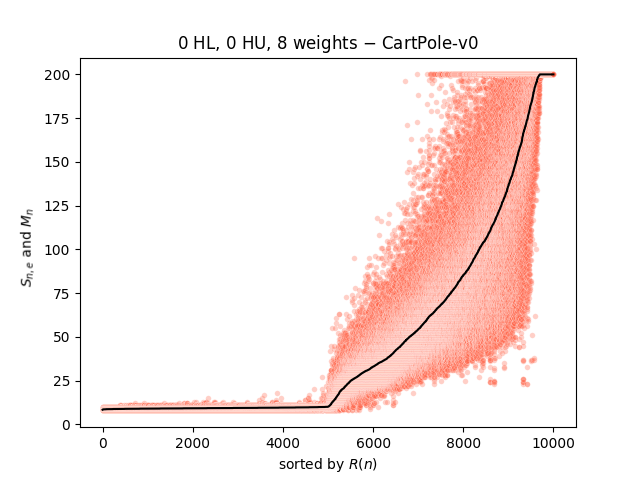
\includegraphics[width=.3\linewidth]{NN/CartPole_NN_HL_0_HU_0_scatter_score.png}
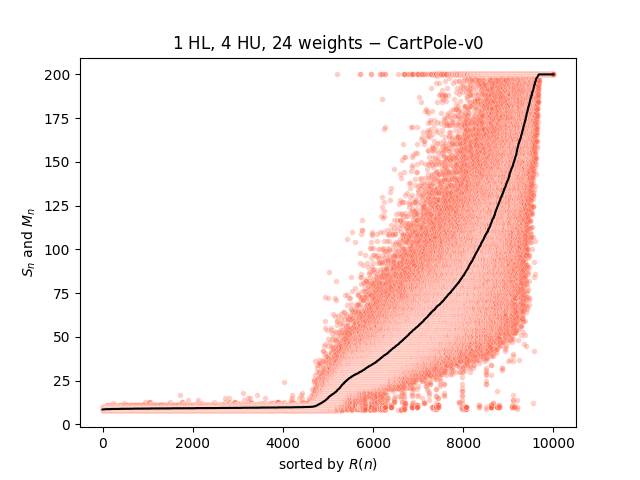
\includegraphics[width=.3\linewidth]{NN/CartPole_NN_HL_1_HU_4_scatter_score.png}
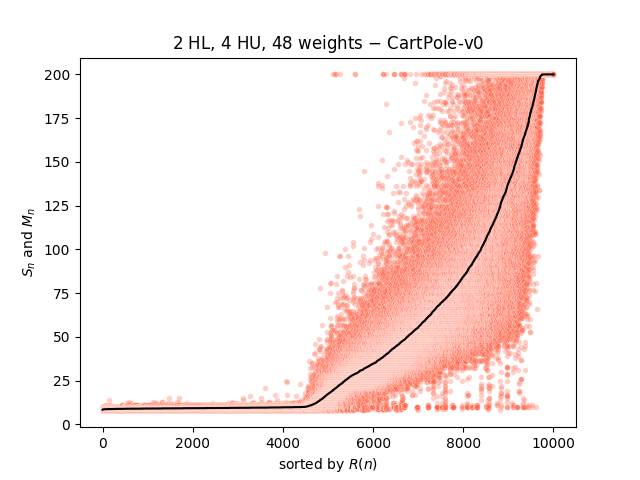
\includegraphics[width=.3\linewidth]{NN/CartPole_NN_HL_2_HU_4_scatter_score.png}}
\item \label{row:NN_Acrobot}  \raisebox{-0.5\height}{
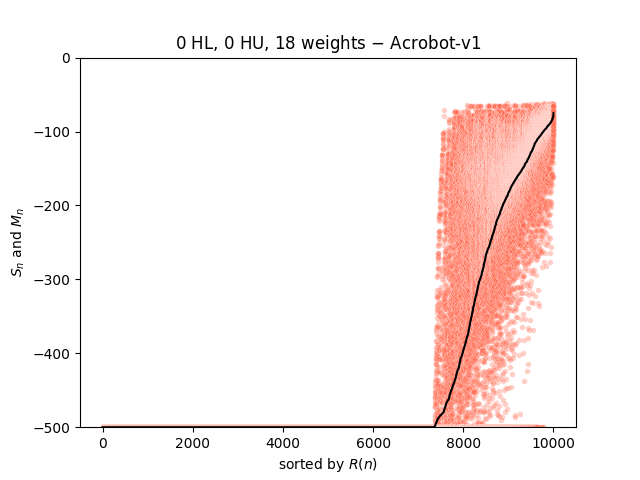
\includegraphics[width=.3\linewidth]{NN/Acrobot_NN_HL_0_HU_0_scatter_score.png}
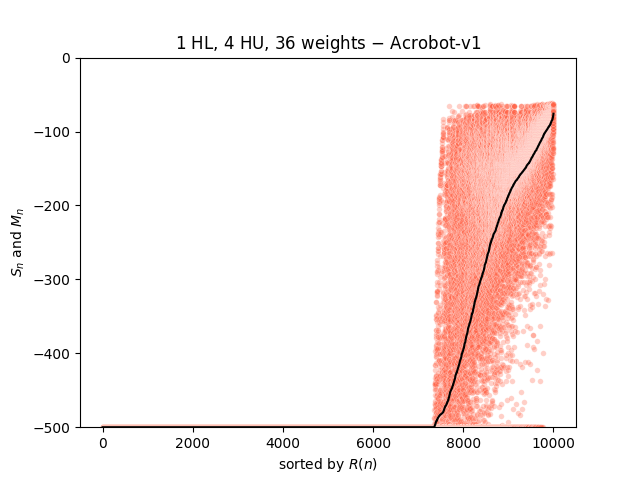
\includegraphics[width=.3\linewidth]{NN/Acrobot_NN_HL_1_HU_4_scatter_score.png}
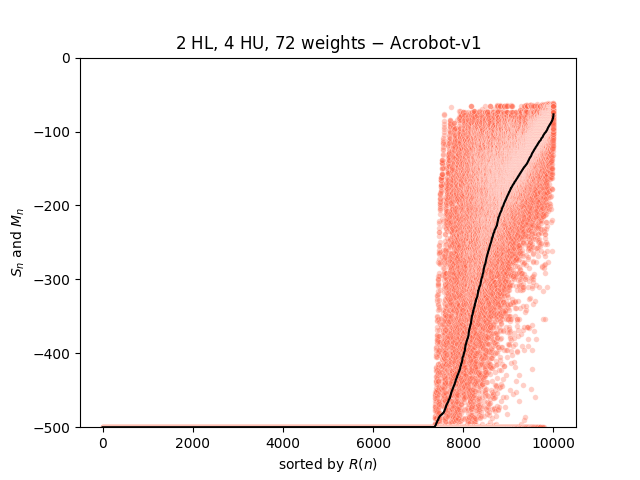
\includegraphics[width=.3\linewidth]{NN/Acrobot_NN_HL_2_HU_4_scatter_score.png}}
\item \label{row:NN_MountainCar}  \raisebox{-0.5\height}{
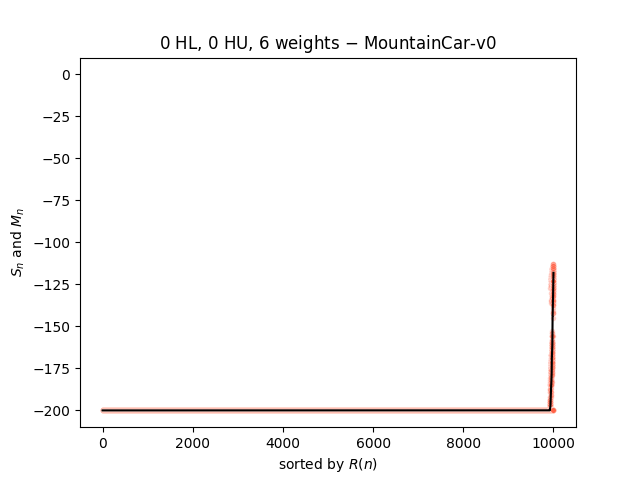
\includegraphics[width=.3\linewidth]{NN/MountainCar_NN_HL_0_HU_0_scatter_score.png}
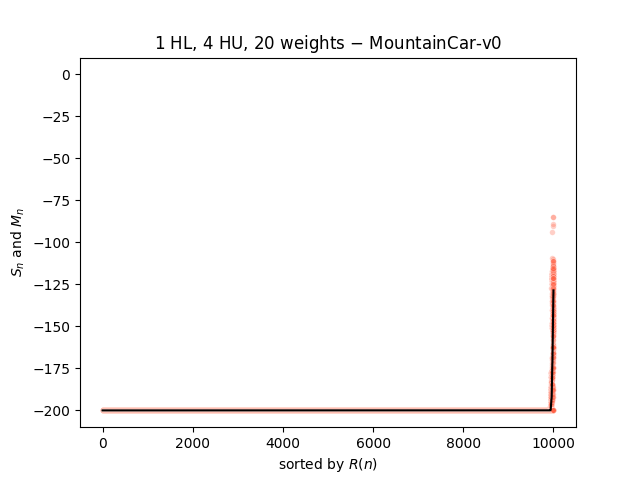
\includegraphics[width=.3\linewidth]{NN/MountainCar_NN_HL_1_HU_4_scatter_score.png}
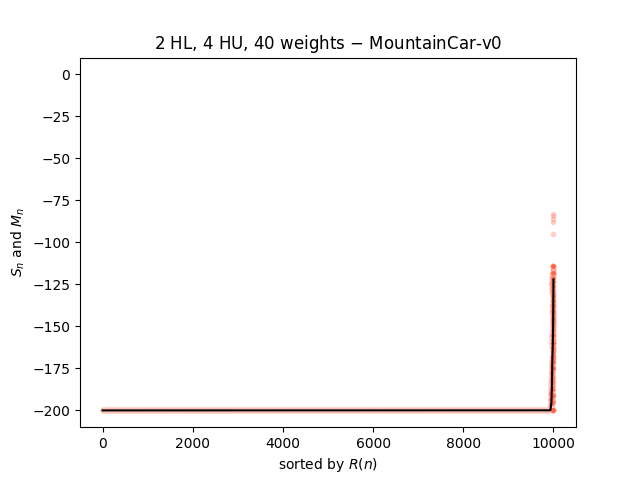
\includegraphics[width=.3\linewidth]{NN/MountainCar_NN_HL_2_HU_4_scatter_score.png}}
\item \label{row:NN_MountainCarCont}  \raisebox{-0.5\height}{
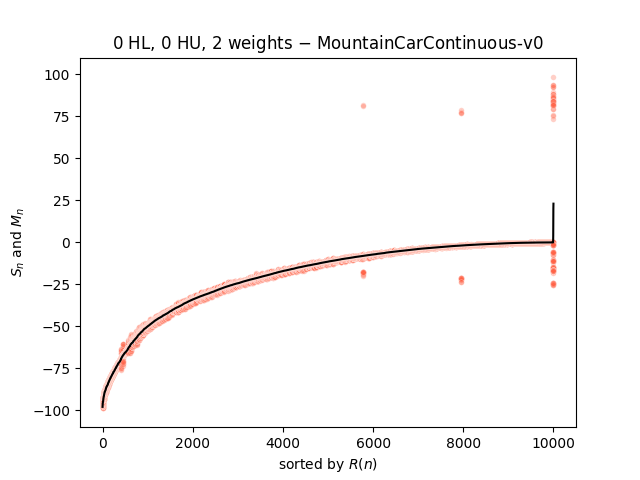
\includegraphics[width=.3\linewidth]{NN/MountainCarCont_NN_HL_0_HU_0_scatter_score.png}
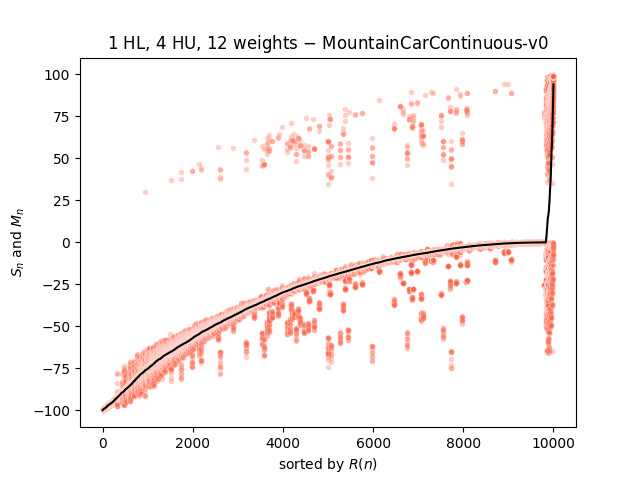
\includegraphics[width=.3\linewidth]{NN/MountainCarCont_NN_HL_1_HU_4_scatter_score.png}
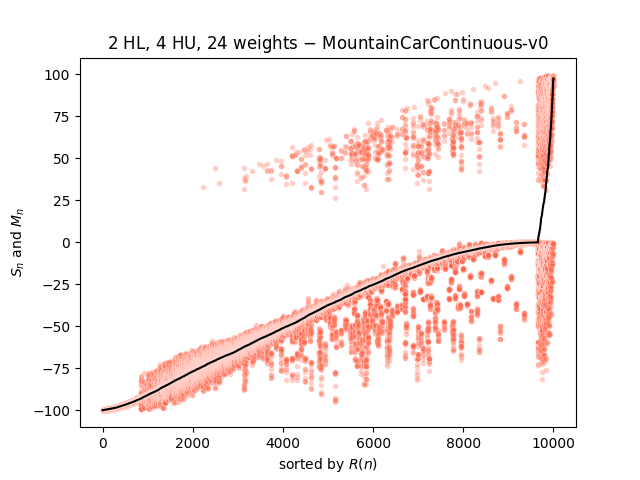
\includegraphics[width=.3\linewidth]{NN/MountainCarCont_NN_HL_2_HU_4_scatter_score.png}}
\item \label{row:NN_Pendulum}  \raisebox{-0.5\height}{
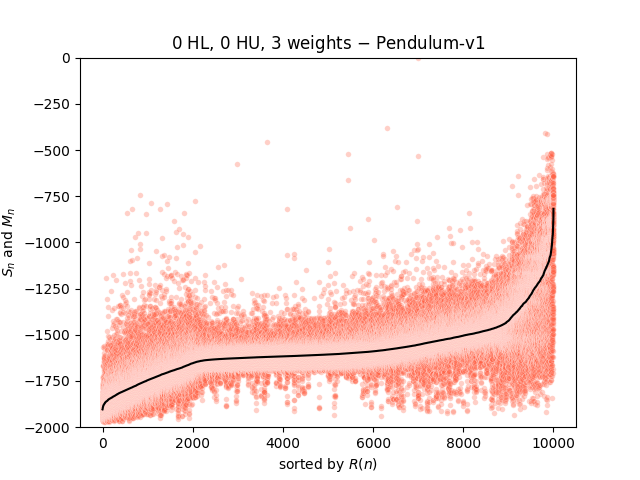
\includegraphics[width=.3\linewidth]{NN/Pendulum_NN_HL_0_HU_0_scatter_score.png}
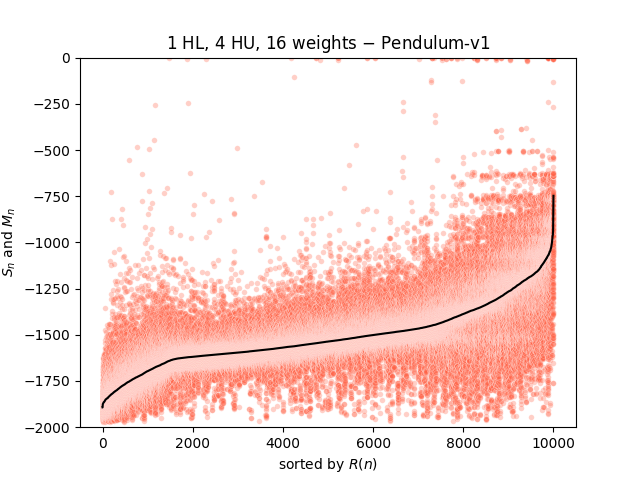
\includegraphics[width=.3\linewidth]{NN/Pendulum_NN_HL_1_HU_4_scatter_score.png}
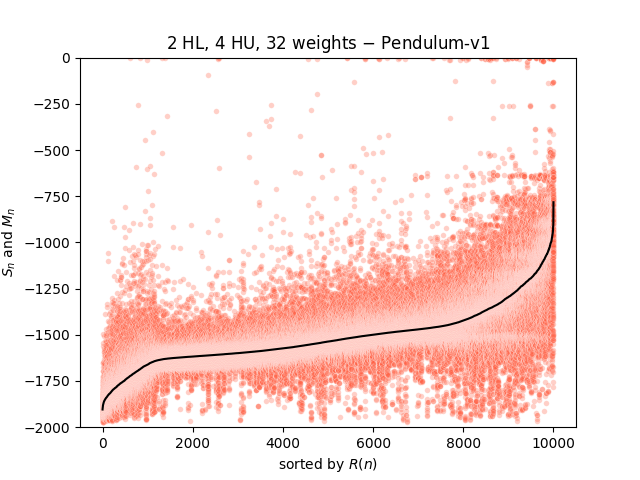
\includegraphics[width=.3\linewidth]{NN/Pendulum_NN_HL_2_HU_4_scatter_score.png}}
\end{figrow}
\caption[Results for all classic control environments using neural networks without bias]{
  \textbf{Results for all classic control environments using neural networks without bias.}
   Each row shows the results of one environment, whereas the columns represent the different network architectures. These plots are a reproduction of the results of the RWG-paper. My results are consistent with those shown in the paper.
}
\label{fig:results_NN}
\end{figure}
For each plot, the samples are ranked according to their mean score and aligned on the $x-$axis according to their rank. The scatter plots show all scores of the samples, whereas the lineplot illustrates the mean of each sample over all episodes. Each column shows a different network architecture. The first column shows the results of the networks without hidden layers, the second column the networks with one hidden layer, and the last column the networks with two hidden layers. The rows are dedicated to the different classic control environments. These results are consistent with the ones from the paper \emph{Analyzing Reinforcement Learning Benchmarks with Random Weight Guessing}. In the subsequent sections, I will refer to these plots to compare the effectiveness of other models or configurations to these neural network architectures.

\subsection{Polynomial Model}
Figure~\ref{fig:results_Polynomial} shows the results for the discrete classic control environments using the polynomial model $P_1$ without bias. The visualization is identical to the one I used for the neural networks in Figure~\ref{fig:results_NN}. The rows show the results for the different environments, and the columns show the polynomial with degrees 1, 2, and 3.
\begin{figure}[!ht]
\begin{figrow}
\item \label{row:Polynomial_CartPole}  \raisebox{-0.5\height}{
\includegraphics[width=.3\linewidth]{PolynomialNN/without_bias/CartPole-v0_PolynomialNN_degree_1_scatter_score}
\includegraphics[width=.3\linewidth]{PolynomialNN/without_bias/CartPole-v0_PolynomialNN_degree_2_scatter_score}
\includegraphics[width=.3\linewidth]{PolynomialNN/without_bias/CartPole-v0_PolynomialNN_degree_3_scatter_score}}
\item \label{row:Polynomial_Acrobot}  \raisebox{-0.5\height}{
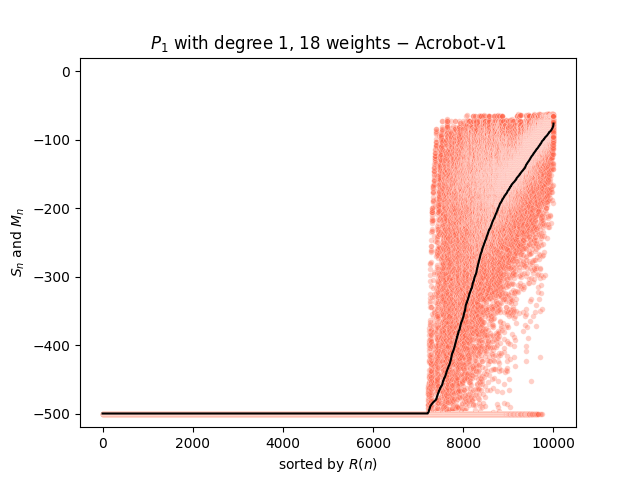
\includegraphics[width=.3\linewidth]{PolynomialNN/without_bias/Acrobot-v1_PolynomialNN_degree_1_scatter_score}
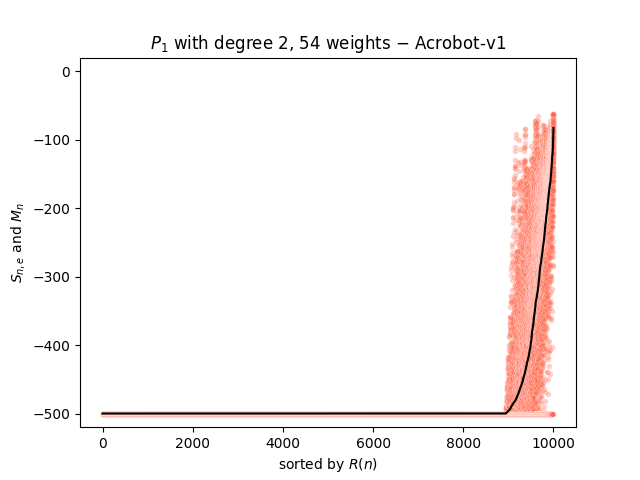
\includegraphics[width=.3\linewidth]{PolynomialNN/without_bias/Acrobot-v1_PolynomialNN_degree_2_scatter_score}
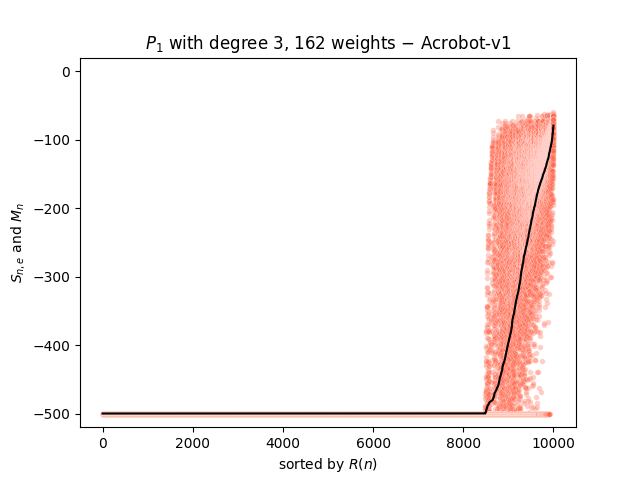
\includegraphics[width=.3\linewidth]{PolynomialNN/without_bias/Acrobot-v1_PolynomialNN_degree_3_scatter_score}}
\item \label{row:Polynomial_MountainCar}  \raisebox{-0.5\height}{
\includegraphics[width=.3\linewidth]{PolynomialNN/without_bias/MountainCar-v0_PolynomialNN_degree_1_scatter_score}
\includegraphics[width=.3\linewidth]{PolynomialNN/without_bias/MountainCar-v0_PolynomialNN_degree_2_scatter_score}
\includegraphics[width=.3\linewidth]{PolynomialNN/without_bias/MountainCar-v0_PolynomialNN_degree_3_scatter_score}}
\end{figrow}
\caption[Results for the discrete classic control environments using the polynomial model $\mathbf{P_1}$ without bias]{
  \textbf{Results for the discrete classic control environments using the polynomial model $\mathbf{P_1}$ without bias.}
   Each row shows the results of one environment. The columns represent the different degrees of the polynomials. In these plots, the model $P_1$ was used. The results aligned in the first column are almost indistinguishable from the ones of the neural networks without hidden layers. Nonetheless, the environments \texttt{CartPole} and \texttt{Acrobot} deliver different results for a higher degree of the polynomial.
}
\label{fig:results_Polynomial}
\end{figure}
Looking at the first column, we can see a striking resemblance to the performance of the neural network without hidden layers shown in Section~\ref{fig:results_NN} for all three environments. This observation is not entirely a surprise since the neural network without hidden layers represents a linear controller. However, the second and last columns show different results for the environments \verb|CartPole| and \verb|Acrobot|.

For the environment \verb|CartPole|, we can see that the curve of the mean score stays low until around $5'000$ but then goes up relatively steeply. That means the linear model fails around 50\% to guess the action correctly. However, after that, we have a high probability to achieve a good score or even solve the task entirely during multiple episodes. There are also quite a few samples that could solve the task each time, as indicated by the short straight black line at the top of the plot. Looking at the polynomials with degree 2 for \verb|CartPole|, we can see that the scores increase already at around $2'000$, but the slope is less steep than for the linear model. Therefore, we start earlier to get meaningful results, but the scores increase only slowly. This aspect is significant for a learning algorithm. In addition, there are fewer samples that could solve the task for each episode than there are for the linear model. Furthermore, the variance is higher for the polynomials with a higher degree compared to the linear model. If we look at the results of the polynomials with degree 3, we can see that there is only a tiny boost compared to the polynomials of degree 2. The scores are overall slightly higher, but the slope is similar to before. The considerable difference lies between the polynomials with degree 1 and polynomials with degree 2, respectively, degree 3.

For the environment \verb|Acrobot|, the lineplot stays at -500 until around rank 7'500 for the linear model. Then it goes up steeply. Thus, we have a large plateau of minimum scores before we reach scores over -500. That opposes a higher difficulty level for the learning algorithm than \verb|CartPole|. But with RWG, we can still reach relatively high scores, and the lineplot is continuous. Interestingly, the polynomial models with a higher degree performed noticeably worse. This observation cannot be made for the neural networks.

The environment \verb|MountainCar| is more challenging to solve than the other environments, as we can see by the results of both the neural networks and the polynomial model. Both models show very similar findings. There is a large fitness plateau, and only a few samples can reach a score higher than the minimum score of -200. That applies to both the linear models and the ones with higher complexity.

Figure~\ref{fig:results_Polynomial_bias} shows the results of using the polynomial model $P_1$ to solve the discrete classic control environments using bias.
\begin{figure}[!ht]
\begin{figrow}
\item \label{row:Polynomial_CartPole_bias}  \raisebox{-0.5\height}{
\includegraphics[width=.3\linewidth]{PolynomialNN/with_bias/CartPole-v0_PolynomialNN_degree_1_scatter_score}
\includegraphics[width=.3\linewidth]{PolynomialNN/with_bias/CartPole-v0_PolynomialNN_degree_2_scatter_score}
\includegraphics[width=.3\linewidth]{PolynomialNN/with_bias/CartPole-v0_PolynomialNN_degree_3_scatter_score}}
\item \label{row:Polynomial_MountainCar_bias}  \raisebox{-0.5\height}{
\includegraphics[width=.3\linewidth]{PolynomialNN/with_bias/MountainCar-v0_PolynomialNN_degree_1_scatter_score}
\includegraphics[width=.3\linewidth]{PolynomialNN/with_bias/MountainCar-v0_PolynomialNN_degree_2_scatter_score}
\includegraphics[width=.3\linewidth]{PolynomialNN/with_bias/MountainCar-v0_PolynomialNN_degree_3_scatter_score}}
\end{figrow}
\caption[Results for the discrete classic control environments using the polynomial model $\mathbf{P_1}$ with bias]{
  \textbf{Results for the discrete classic control environments using the polynomial model $\mathbf{P_1}$ with bias.}
   Each row shows the results of one environment. The columns represent the different degrees of the polynomials. For these plots, the polynomial model $P_1$ was used. Overall, the model performs noticeably worse with bias as opposed to without bias.
}
\label{fig:results_Polynomial_bias}
\end{figure}
Comparing these results with the ones without using bias in Figure~\ref{fig:results_Polynomial} shows a significant difference. The bias influences the performance of the model negatively. Thus, the observation about the bias that the authors made in the paper \emph{Analyzing Reinforcement Learning Benchmarks with Random Weight Guessing} is not specific to neural networks but seems to be more of a general factor.

%Figure~\ref{fig:experiment_1_polynomial} shows the results of the first experiment for the two architectures of the polynomial model $P_1$ and $P_2$. I visualized the results of each model with bias connection in row (a) and without bias connection in row (b). The structure of the plots is identical for better comparison. The samples are ranked according to their mean score and aligned on the $x-$axis according to their rank. The scatter plots show all scores of the samples, whereas the lineplot illustrates the mean of each sample over all episodes. Subfigure~\ref{fig:results_p1} shows the results of the polynomial model $P_1$ and Subfigure~\ref{fig:results_p2} shows the results of the polynomial model $P_2$.
%\begin{figure}[!ht]
%\begin{subfigure}{\textwidth}
%\begin{figrow}
%\item \label{row:P1_with_bias} \raisebox{-0.5\height}{
%\includegraphics[width=.3\linewidth]{experiment_1/with_bias/PolynomialNN_degree_1_scatter_score.png}
%\includegraphics[width=.3\linewidth]{experiment_1/with_bias/PolynomialNN_degree_2_scatter_score.png}
%\includegraphics[width=.3\linewidth]{experiment_1/with_bias/PolynomialNN_degree_3_scatter_score.png}}
%\item \label{row:P1_without_bias}  \raisebox{-0.5\height}{
%\includegraphics[width=.3\linewidth]{experiment_1/without_bias/PolynomialNN_degree_1_scatter_score.png}
%\includegraphics[width=.3\linewidth]{experiment_1/without_bias/PolynomialNN_degree_2_scatter_score.png}
%\includegraphics[width=.3\linewidth]{experiment_1/without_bias/PolynomialNN_degree_3_scatter_score.png}}
%\end{figrow}
%\vspace*{-5mm}
%\caption{Results of $P_1$ with bias (a) and without bias (b)}
%\label{fig:results_p1}
%\end{subfigure}
%\begin{subfigure}{\textwidth}
%\begin{figrow}
%\item \label{row:P2_with_bias} \raisebox{-0.5\height}{
%\includegraphics[width=.3\linewidth]{experiment_1/with_bias/Polynomial_degree_1_scatter_score.png}
%\includegraphics[width=.3\linewidth]{experiment_1/with_bias/Polynomial_degree_2_scatter_score.png}
%\includegraphics[width=.3\linewidth]{experiment_1/with_bias/Polynomial_degree_3_scatter_score.png}}
%\item \label{row:P2_without_bias}  \raisebox{-0.5\height}{
%\includegraphics[width=.3\linewidth]{experiment_1/without_bias/Polynomial_degree_1_scatter_score.png}
%\includegraphics[width=.3\linewidth]{experiment_1/without_bias/Polynomial_degree_2_scatter_score.png}
%\includegraphics[width=.3\linewidth]{experiment_1/without_bias/Polynomial_degree_3_scatter_score.png}}
%\end{figrow}
%\vspace*{-5mm}
%\caption{Results of $P_2$ with bias (a) and without bias (b)}
%\label{fig:results_p2}
%\end{subfigure}
%\caption[Results of experiment 1: polynomial models]{
%  \textbf{Results of experiment 1: polynomial models.}
%   The figures show the results of the first experiment with the two polynomial models. On the $x-$axis, we have the rank of each sample. On the $y-$axis, we have the scores of all samples and the mean as a lineplot. Each subplot shows the performance of the model with bias in row (a) and without bias in row (b). As we can see, both models perform equally good or bad. However, there is a huge difference in performance whether we are working with or without bias. In addition, we can see a difference in the slope of the mean values between polynomials with degree 1 and one with a higher degree.
%}
%\label{fig:experiment_1_polynomial}
%\end{figure}
%As we can see in the images, the plots of the two models almost look identical. Both models performed equally good or bad despite their different architecture and the different number of weights. Because of this similarity, I will not go into each model independently but instead discuss further results for both of them. There is only a little difference between the two models even though the weights are doubled for $P_1$ and a half more for $P_2$. It seems that the complexity of the model depends more on the architecture of the model than on the number of weights.


\todo[inline]{Add missing plots for bias. Include plots of $P_2$ as well (failed for MountainCar)?}

\subsection{Binary Tree Model}
For the binary trees, I tested three models, one with 1 node, one with 4 nodes, and one with 8 nodes. Since the previous experiments suggest that using bias has a negative effect, the following experiments do not include bias. Figure~\ref{fig:results_BinaryTree} shows the results for all five classic control environments with the binary tree model.
\begin{figure}[!ht]
\begin{figrow}
\item \label{row:BinaryTree_CartPole} \raisebox{-0.5\height}{
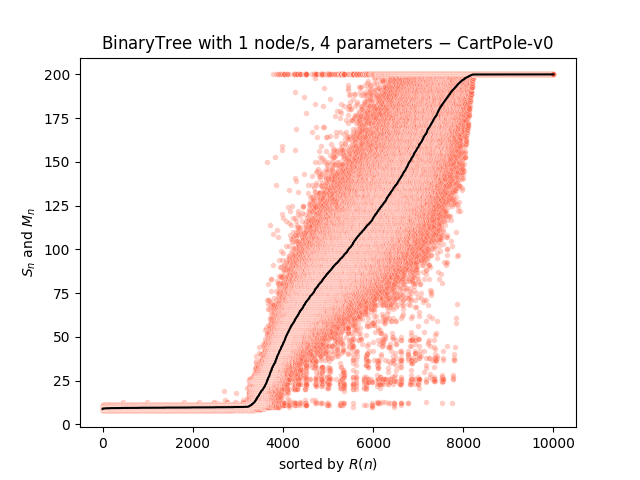
\includegraphics[width=.3\linewidth]{Binary_Tree/CartPole_BinaryTree_1_nodes_scatter_score.png}
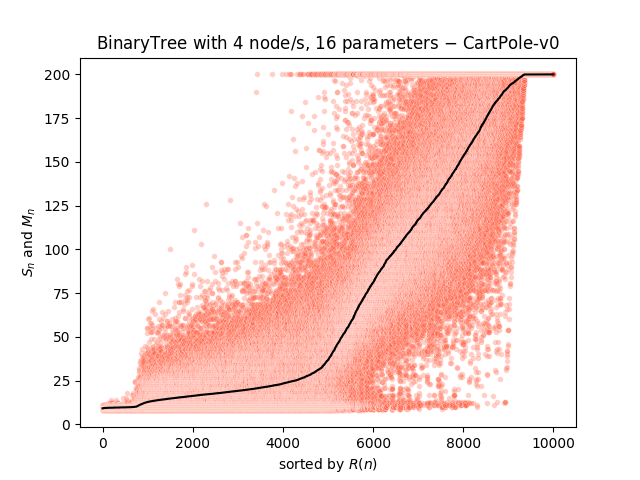
\includegraphics[width=.3\linewidth]{Binary_Tree/CartPole_BinaryTree_4_nodes_scatter_score.png}
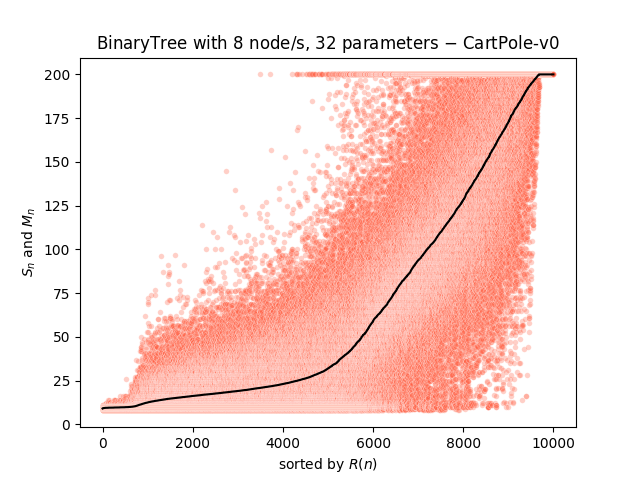
\includegraphics[width=.3\linewidth]{Binary_Tree/CartPole_BinaryTree_8_nodes_scatter_score.png}}
\item \label{row:BinaryTree_Acrobot} \raisebox{-0.5\height}{
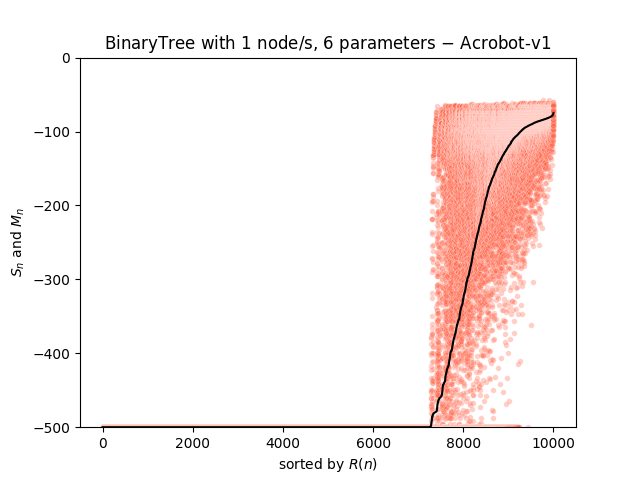
\includegraphics[width=.3\linewidth]{Binary_Tree/Acrobot_BinaryTree_1_nodes_scatter_score.png}
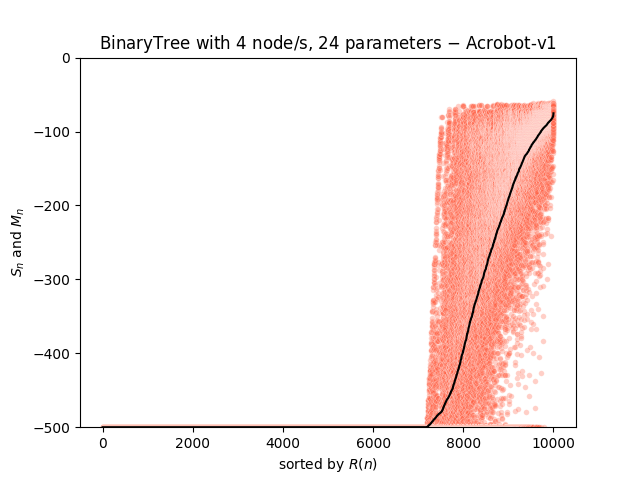
\includegraphics[width=.3\linewidth]{Binary_Tree/Acrobot_BinaryTree_4_nodes_scatter_score.png}
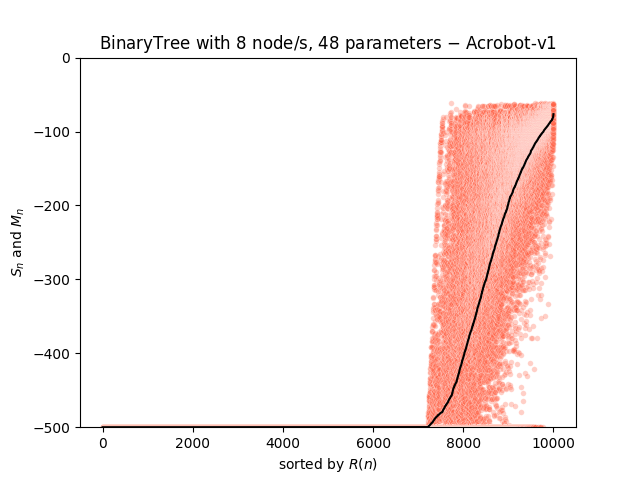
\includegraphics[width=.3\linewidth]{Binary_Tree/Acrobot_BinaryTree_8_nodes_scatter_score.png}}
\item \label{row:BinaryTree_MountainCar} \raisebox{-0.5\height}{
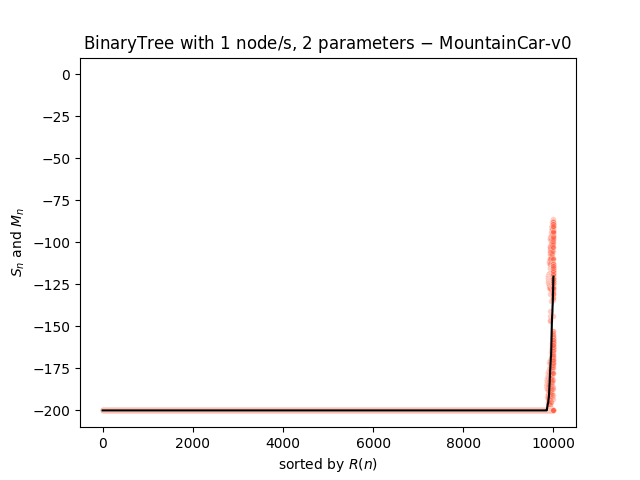
\includegraphics[width=.3\linewidth]{Binary_Tree/MountainCar_BinaryTree_1_nodes_scatter_score.png}
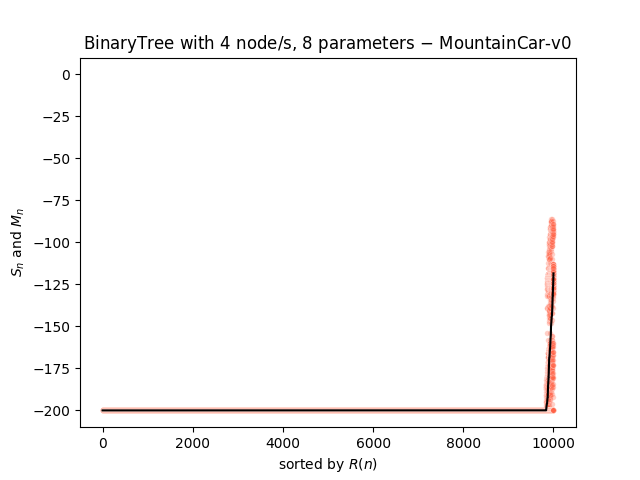
\includegraphics[width=.3\linewidth]{Binary_Tree/MountainCar_BinaryTree_4_nodes_scatter_score.png}
\includegraphics[width=.3\linewidth]{Binary_Tree/MountainCar_BinaryTree_8_nodes_scatter_score.png}}
\item \label{row:BinaryTree_MountainCarCont}  \raisebox{-0.5\height}{
\includegraphics[width=.3\linewidth]{Binary_Tree/MountainCarCont_BinaryTree_1_nodes_scatter_score.png}
\includegraphics[width=.3\linewidth]{Binary_Tree/MountainCarCont_BinaryTree_4_nodes_scatter_score.png}
\includegraphics[width=.3\linewidth]{Binary_Tree/MountainCarCont_BinaryTree_8_nodes_scatter_score.png}}
\item \label{row:BinaryTree_Pendulum} \raisebox{-0.5\height}{
\includegraphics[width=.3\linewidth]{Binary_Tree/Pendulum_BinaryTree_1_nodes_scatter_score.png}
\includegraphics[width=.3\linewidth]{Binary_Tree/Pendulum_BinaryTree_4_nodes_scatter_score.png}
\includegraphics[width=.3\linewidth]{Binary_Tree/Pendulum_BinaryTree_8_nodes_scatter_score.png}}
\end{figrow}
\caption[Results for the classic control environments using binary trees without bias]{
  \textbf{Results for the classic control environments using binary trees without bias.}
   Each row shows the results of one environment. The columns represent the different configurations for the binary tree models. Even with only one node, the results are comparable to those from neural networks or outperform them.
}
\label{fig:results_BinaryTree}
\end{figure}

Comparing the results using binary trees with those using neural networks shown in Figure~\ref{fig:results_NN}, we can see a few differences. For the environment \verb|CartPole|, we can see that we generally reach  better scores with the binary trees. Comparing the neural network without hidden layers with the binary tree with only one node, we have a similar curve, but the lineplot representing the mean scores sets off much earlier at around 3'500 for the binary tree than the one for the neural network, which sets off at around 5'000. In addition, the binary tree has a higher chance of reaching a maximal mean score, indicated by the straight black line at the top right. For the more complex architectures, it gets more interesting. The binary tree with four nodes can already raise the mean value under 1'000 samples. That tells us that the problem of the fitness plateau is reduced significantly. Thus, when using a learning algorithm, the binary tree has a better chance of solving the problem without getting stuck in a fitness plateau. The chance of reaching a maximal mean score decreases with adding more nodes to the binary tree. That could be caused by the increasing complexity of the binary tree, which makes it harder to guess the weights correctly. Furthermore, the scores are more spread out for the binary trees than for the neural networks, indicating a higher variance.

For the environment \verb|Acrobot|, the plots do not show a significant difference between the two models. Overall, we can say that both models reach similar scores and mean values. However, the scores seem to be more spread out for the binary trees than for the neural networks, resulting in a higher variance.

The \verb|MountainCar| environment is more challenging for a learning algorithm. Comparing the two models, binary trees and neural networks, we can see that the binary trees are more likely to reach a better score. However, the risk of being stuck in a fitness plateau remains. In addition, the scores are spread wider for the binary tree than for the neural network.

The results for the environment \verb|MountainCarContinuous| look very different for the binary trees than for the neural networks. Neural networks show a slowly increasing curve with a peak for the mean scores. The binary trees have a lot of low performers. However, there are a few samples that are able to reach a positive score. The neural network without hidden layers could not achieve these high mean scores. The considerable difference between the two models could be caused by the binary tree still producing discrete actions instead of continuous ones, as neural networks did. For the binary tree model, the action is either -1 or 1, limiting the output space significantly.

For the \verb|Pendulum| environment, we can see that the binary trees perform increasingly better with more nodes. The difference between the two models, neural network and binary tree, is not huge. However, we can see that using neural networks results in a few higher mean scores. But with the binary trees, we have a slightly higher score in the middle area. Additionally, the binary trees show a higher variance than the neural networks. Even though the actions produced by the binary trees are discrete instead of continuous, the curve of the mean scores looks very similar to the one produced by neural networks.

\todo[inline]{Explain how model handeled continuous environments in models section.}

\subsection{Bias Investigation}
In their paper, \citet{oller_analyzing_2020} mentioned that using bias negatively affects the score distribution leading to fewer top performers and generally lower scores. Figure~\ref{fig:results_NN_bias} shows my results for all classic control environments with neural networks without using bias.
\begin{figure}[!ht]
\begin{figrow}
\item \label{row:NN_with_bias_CartPole} \raisebox{-0.5\height}{
\includegraphics[width=.3\linewidth]{experiment_2/default/with_bias/CartPole-v0_NN_HL_0_HU_0_scatter_score}
\includegraphics[width=.3\linewidth]{experiment_2/default/with_bias/CartPole-v0_NN_HL_1_HU_4_scatter_score}
\includegraphics[width=.3\linewidth]{experiment_2/default/with_bias/CartPole-v0_NN_HL_2_HU_4_scatter_score}}
\item \label{row:NN_with_bias_Acrobot} \raisebox{-0.5\height}{
\includegraphics[width=.3\linewidth]{experiment_2/default/with_bias/Acrobot-v1_NN_HL_0_HU_0_scatter_score}
\includegraphics[width=.3\linewidth]{experiment_2/default/with_bias/Acrobot-v1_NN_HL_1_HU_4_scatter_score}
\includegraphics[width=.3\linewidth]{experiment_2/default/with_bias/Acrobot-v1_NN_HL_2_HU_4_scatter_score}}
\item \label{row:NN_with_bias_MountainCar} \raisebox{-0.5\height}{
\includegraphics[width=.3\linewidth]{experiment_2/default/with_bias/MountainCar-v0_NN_HL_0_HU_0_scatter_score}
\includegraphics[width=.3\linewidth]{experiment_2/default/with_bias/MountainCar-v0_NN_HL_1_HU_4_scatter_score}
\includegraphics[width=.3\linewidth]{experiment_2/default/with_bias/MountainCar-v0_NN_HL_2_HU_4_scatter_score}}
\item \label{row:NN_with_bias_MountainCarCont} \raisebox{-0.5\height}{
\includegraphics[width=.3\linewidth]{experiment_2/default/with_bias/MountainCarContinuous-v0_NN_HL_0_HU_0_scatter_score}
\includegraphics[width=.3\linewidth]{experiment_2/default/with_bias/MountainCarContinuous-v0_NN_HL_1_HU_4_scatter_score}
\includegraphics[width=.3\linewidth]{experiment_2/default/with_bias/MountainCarContinuous-v0_NN_HL_2_HU_4_scatter_score}}
\item \label{row:NN_with_bias_Pendulum} \raisebox{-0.5\height}{
\includegraphics[width=.3\linewidth]{experiment_2/default/with_bias/Pendulum-v1_NN_HL_0_HU_0_scatter_score}
\includegraphics[width=.3\linewidth]{experiment_2/default/with_bias/Pendulum-v1_NN_HL_1_HU_4_scatter_score}
\includegraphics[width=.3\linewidth]{experiment_2/default/with_bias/Pendulum-v1_NN_HL_2_HU_4_scatter_score}}
\end{figrow}
\caption[Results for all classic control environments using neural networks with bias]{
  \textbf{Results for all classic control environments using neural networks with bias.}
   Each row shows the results of one environment, whereas the columns represent the different network architectures. For most environments, we can see that introducing a bias has a negative effect on the score distribution.
}
\label{fig:results_NN_bias}
\end{figure}
Comparing these plots with the ones without using bias in Figure~\ref{fig:results_NN}, we can see the negative impact the bias has on the effectiveness of the model. For the environment \verb|CartPole|, the scores are overall lower and get slighly worse with the increased complexity of the model. Interestingly, for the environment \verb|Acrobot|, the network without hidden layers is resistent to the negative impact of the bias. However, the network with one hidden layer results in lower scores with bias. The network with two hidden layers with has slightly better results than the one with one hidden layer but still performs worse than the one without bias. The same observation can be made for the environment \verb|MountainCar|. For the environment \verb|MountainCarContinuous|, we can see a negative effect on the score distribution for all three network architectures. The environment \verb|Pendulum| does not seem to suffer much when introducing bias. For all three architectures, there is not much difference visible. The scores are generally lower and produce less top performers when using bias. Therefore, we can confirm the interesting observation of the authors, namely, that using bias is counterproductive in this experimental setting.

To further investigate this behavior, Figure~\ref{fig:results_NN_weights} shows the results of tripling the number of weights for each network architecture for all classic control environments.
\begin{figure}[!ht]
\begin{figrow}
\item \label{row:NN_CartPole_wfactor_3}  \raisebox{-0.5\height}{
\includegraphics[width=.3\linewidth]{experiment_2/weights/weight_factor_3/without_bias/CartPole-v0_NN_HL_0_HU_0_scatter_score}
\includegraphics[width=.3\linewidth]{experiment_2/weights/weight_factor_3/without_bias/CartPole-v0_NN_HL_1_HU_4_scatter_score}
\includegraphics[width=.3\linewidth]{experiment_2/weights/weight_factor_3/without_bias/CartPole-v0_NN_HL_2_HU_4_scatter_score}}
\item \label{row:NN_Acrobot_wfactor_3}  \raisebox{-0.5\height}{
\includegraphics[width=.3\linewidth]{experiment_2/weights/weight_factor_3/without_bias/Acrobot-v1_NN_HL_0_HU_0_scatter_score}
\includegraphics[width=.3\linewidth]{experiment_2/weights/weight_factor_3/without_bias/Acrobot-v1_NN_HL_1_HU_4_scatter_score}
\includegraphics[width=.3\linewidth]{experiment_2/weights/weight_factor_3/without_bias/Acrobot-v1_NN_HL_2_HU_4_scatter_score}}
\item \label{row:NN_MountainCar_wfactor_3}  \raisebox{-0.5\height}{
\includegraphics[width=.3\linewidth]{experiment_2/weights/weight_factor_3/without_bias/MountainCar-v0_NN_HL_0_HU_0_scatter_score}
\includegraphics[width=.3\linewidth]{experiment_2/weights/weight_factor_3/without_bias/MountainCar-v0_NN_HL_1_HU_4_scatter_score}
\includegraphics[width=.3\linewidth]{experiment_2/weights/weight_factor_3/without_bias/MountainCar-v0_NN_HL_2_HU_4_scatter_score}}
\item \label{row:NN_Pendulum_wfactor_3}  \raisebox{-0.5\height}{
\includegraphics[width=.3\linewidth]{experiment_2/weights/weight_factor_3/without_bias/Pendulum-v1_NN_HL_0_HU_0_scatter_score}
\includegraphics[width=.3\linewidth]{experiment_2/weights/weight_factor_3/without_bias/Pendulum-v1_NN_HL_1_HU_4_scatter_score}
\includegraphics[width=.3\linewidth]{experiment_2/weights/weight_factor_3/without_bias/Pendulum-v1_NN_HL_2_HU_4_scatter_score}}
\end{figrow}
\vspace*{-5mm}
\caption[Results of tripling the number of weights for neural networks]{
  \textbf{Results of tripling the number of weights for neural networks.}
   The figure shows the results of tripling the number of weights for the three neural network architectures for the classic control environments. Despite the increased number of weights, there is no visible difference in the plots compared to the ones shown in Figure~\ref{fig:results_NN}.
}
\label{fig:results_NN_weights}
\end{figure}
Comparing these plots to those in Figure~\ref{fig:results_NN}, we can barely see a difference. The slope of the mean values looks the same. The data points do not show different behavior. Thus, we can conclude that increasing the number of weights does not impact the achieved score of the model significantly.
%In addition, the same experiment with the polynomial models $P_1$ and $P_2$ draws the same conclusion.

Figure~\ref{fig:experiment_2_layers} shows the results of altering the number of layers in a network.
%For the networks with bias connections, the performance gets significantly worse with an increased number of layers. The networks without bias connections seem to be more robust. Still, the steepness of the slope of the line plots decreases with an increased number of layers.
\begin{figure}[!ht]
\begin{figrow}
\item \label{row:NN_CartPole_layers}  \raisebox{-0.5\height}{
\includegraphics[width=.3\linewidth]{experiment_2/layers/without_bias/CartPole-v0_NN_HL_4_HU_4_scatter_score}
\includegraphics[width=.3\linewidth]{experiment_2/layers/without_bias/CartPole-v0_NN_HL_6_HU_4_scatter_score}
\includegraphics[width=.3\linewidth]{experiment_2/layers/without_bias/CartPole-v0_NN_HL_8_HU_4_scatter_score}}
\item \label{row:NN_MountainCar_layers}  \raisebox{-0.5\height}{
\includegraphics[width=.3\linewidth]{experiment_2/layers/without_bias/MountainCar-v0_NN_HL_4_HU_4_scatter_score}
\includegraphics[width=.3\linewidth]{experiment_2/layers/without_bias/MountainCar-v0_NN_HL_6_HU_4_scatter_score}
\includegraphics[width=.3\linewidth]{experiment_2/layers/without_bias/MountainCar-v0_NN_HL_8_HU_4_scatter_score}}
\item \label{row:NN_MountainCarContinuous_layers}  \raisebox{-0.5\height}{
\includegraphics[width=.3\linewidth]{experiment_2/layers/without_bias/MountainCarContinuous-v0_NN_HL_4_HU_4_scatter_score}
\includegraphics[width=.3\linewidth]{experiment_2/layers/without_bias/MountainCarContinuous-v0_NN_HL_6_HU_4_scatter_score}
\includegraphics[width=.3\linewidth]{experiment_2/layers/without_bias/MountainCarContinuous-v0_NN_HL_8_HU_4_scatter_score}}
\end{figrow}
\caption[Results of altering the number of layers for neural networks]{
  \textbf{Results of altering the number of layers for neural networks.}
   The plots show the result of increasing the number of hidden layers gradually.
}
\label{fig:experiment_2_layers}
\end{figure}

Figure~\ref{fig:experiment_2_neurons} shows the results of increasing the number of neurons in each hidden layer for a network with two hidden layers. Comparing the plots with the ones in Figure~\ref{fig:results_NN}, the results do not show much difference. The slope is a little less steep with increased neurons.
\begin{figure}[!ht]
\begin{figrow}
\item \label{row:NN_with_bias_neurons} \raisebox{-0.5\height}{
\includegraphics[width=.3\linewidth]{experiment_2/neurons/with_bias/HL_2_HU_5_scatter_score.png}
\includegraphics[width=.3\linewidth]{experiment_2/neurons/with_bias/HL_2_HU_8_scatter_score.png}
\includegraphics[width=.3\linewidth]{experiment_2/neurons/with_bias/HL_2_HU_10_scatter_score.png}}
\item \label{row:NN_without_neurons}  \raisebox{-0.5\height}{
\includegraphics[width=.3\linewidth]{experiment_2/neurons/without_bias/HL_2_HU_5_scatter_score.png}
\includegraphics[width=.3\linewidth]{experiment_2/neurons/without_bias/HL_2_HU_8_scatter_score.png}
\includegraphics[width=.3\linewidth]{experiment_2/neurons/without_bias/HL_2_HU_10_scatter_score.png}}
\end{figrow}
\caption[Results of experiment 2: neurons]{
  \textbf{Results of experiment 2: neurons.}
  The plots show the result of increasing the number of neurons for each layer in a network with two hidden layers. The plots in row (a) represent the networks with bias connections, the ones in row (b) represent the networks without bias connections. We can see a slight improvement in row (a).
}
\label{fig:experiment_2_neurons}
\end{figure}

\todo[inline]{Restructuring, adjust text, exchange plots. Does it make sense to do all envs. in this experiments?}

\clearpage
\section{Discussion}
This chapter delivered a direct comparison between neural networks and alternative models like polynomials and binary trees. In addition, I investigated the impact of bias in these settings.
\\ \\
\textbf{Comparison of polynomial model with neural networks:}
The polynomial model can definitely deliver comparable results to neural networks for the discrete enviornments. The results of the environment \texttt{MountainCar} with the polynomial model look almost indistinguishable from those of the neural network model. For the environment \texttt{Acrobot} with a higher complexity of the model, neural networks outperform the polynomial model. Nonetheless, for the \texttt{CartPole} environment, the plots differ from neural networks. The mean scores show the same trend for all neural network architectures. This cannot be applied to the polynomial model. With the linear polynomial model, we have a $50 \%$ chance of failing, but the probability of actually solving the task for all episodes is higher than for the polynomials with a higher degree. That means that with the linear model or neural networks, we have a larger fraction of samples that can solve the environment independently of the initialization conditions. At first glance, we could assume that this is an important aspect for such a model and choose the polynomial with degree 1 over one with a higher degree. However, we should remind ourselves that these experiments are rather unusual for an application since there is no learning involved and the number of samples is huge. In a standard application, we would use some kind of training and want the model to sequentially improve its performance. Considering this aspect, when using a learning algorithm, we would not prefer the polynomials with degree 1 as we might get stuck in a fitness plateau when the algorithm has no method of dealing with this behavior.
\\ \\
\textbf{Comparison of binary tree model with neural networks:} Despite the simple structure of the binary tree model, it could deliver comparable results or even outperform neural networks. The binary tree model outperformed neural networks for the environments \verb|CartPole| and \verb|MountainCar|. The results are similar for the two models for the environment \verb|Acrobot|. Even though the binary tree model at its current implementation outputs only discrete action values, the results for the continuous environment \verb|Pendulum| are comparable to those of neural networks. For the environment \verb|MountainCarContinuous|, neural networks delivered better results.
\\ \\
\textbf{Impact of bias:} No other aspect impacted the performance of the model as much negatively as using bias. It seems that this behavior is specific to the bias in the setting of RWG.

\todo[inline]{Explain more.}
